\documentclass[a4paper,11pt]{report} %article

\usepackage{graphicx,subfigure,afterpage,hyperref,xspace,xcolor,caption}

%command to substitute "{\em MyTaxyService}" with "\mts"
\newcommand{\mts}{\mbox{\normalfont\itshape MyTaxiService\ }}



%tOC style: sections bold 
\usepackage[subfigure]{tocloft}
\renewcommand{\cftsecfont}{\bfseries}
\renewcommand{\cftsecpagefont}{\normalfont\bfseries}% page numbers in bold
\renewcommand{\cftdotsep}{1}
\renewcommand{\cftsecleader}{\bfseries\cftdotfill{\cftsecdotsep}}% dot leaders in bold

%to keep the links of the TOC invisible
\hypersetup{
	colorlinks,
	citecolor=black,
	filecolor=black,
	linkcolor=black,
	urlcolor=black
}

%to center the title "Contents" of the TOC
%\renewcommand\cfttoctitlefont{\hfill\Large\bfseries}
%\renewcommand\cftaftertoctitle{\hfill\mbox{}}



\title{Politecnico di Milano\\A.A. 2015/2016\\Software Engineering 2: ``{\em MyTaxyService}''}
\author{Alessandro Baldassari (mat. 841561) \and Alberto Bendin (mat. 841734) \and Francesco Giarola (mat. 840554)}


\hyphenation{MyTaxyService}


\begin{document}
	
	%fIRSTPAGE
	
	%pOLIMI-LOGO
	\begin{figure}[t]
		\centering
%		\includegraphics[width=1\linewidth]{"C:/Users/alber/Dropbox/Software Engineering 2/Project/polimi-logo"}
			\includegraphics[width=1\linewidth]{"Pictures/polimi-logo"}
	%	\caption{}
		\label{fig:polimi-logo}
	\end{figure}
	
	\maketitle
		
	
	%bLANK-PAGE
%	\afterpage{
%		\thispagestyle{empty}
%		\clearpage\null\newpage
%	}

%	\clearpage
	\thispagestyle{empty}
%	\phantom{a}
%	\vfill
	\clearpage\mbox{}\clearpage
%	\newpage
%	\centering[This page intentionally left blank]
%	\vfill
%	\addtocounter{page}{-1}
	
	
	
	%to number the section from 1 instead of 0.1 with the report class, without using the article class. Avoid the forced use of chapters to number from 1. Tailored for REPORT class!!!
	\renewcommand*\thesection{\arabic{section}}
	\renewcommand*\thesubsection{\arabic{section}.\arabic{subsection}}
	\renewcommand*\thesubsubsection{%
		\arabic{section}.\arabic{subsection}.\arabic{subsubsection}%
	}
	\setcounter{secnumdepth}{4}
	\setcounter{tocdepth}{4}
		
	
	%to change the page numbering from roman in the toc to arabic
	\pagenumbering{roman}
	\tableofcontents
	\newpage
	\pagenumbering{arabic}
	
	
	%to insert the writing "Page" above page numbers in the TOC
	\addtocontents{toc}{~\hfill\textrm{Page}\par}
	
	\section{Introduction}
	
	\subsection{Purpose} The purpose of this document is to describe in a complete and sound way
	the \mts application that will be developed and the application domain in which it will run.\\
	The intended audience for this document are the developers and programmers
	who have to implement the application, system and requirement
	analysts who want to integrate \mts with their system or software,
	testers who have to determine whether the requirements have been satisfied in
	the application implementation, projects managers who have to plan, estimate
	and control the analysis and development processes and finally the users themselves.
	This document could be used as a contractual agreement between the costumer
	and the entity who develops the application.
	
	\subsection{Scope} \label{sec:scope}
	\mts is a new web and mobile application conceived to provide an immediate and user-friendly access to the taxi service of a large city; it aims at an overall improvement of the quality of the service offered.\\
	This optimization is obtained thanks to the real-time interaction and feedback of all the parties involved in the service: taxi passengers can choose and book the ride, and the system will forward the request to the nearest available taxi drivers who can decide to take over the call; in this case the system will notify the client with the code of the incoming taxi and the waiting-time.
	The	system	guarantees a fair management of taxi queues. In particular, the city is divided in taxi zones and each zone is associated with its taxi queue. The system automatically computes the distribution of taxis in the various zones based on the GPS information it receives from each taxi. When a taxi is available, its identifier is stored in the queue of taxis in the corresponding zone. When a request arrives from a certain zone, the system forwards it to the taxis in the corresponding zone according to their order in the queue. If the taxi confirms, then the system will send a confirmation to the passenger. If not, then the system will forward the request to the second in queue and will move the first taxi in the last position of the queue.
	Additional features of the application are the possibility for the passengers to reserve a ride with an advance of at least two hours, choosing the origin and destination, and the option to possibly share the ride with someone else, thus dividing the cost of the service. The system confirms the reservation to the user and allocates a taxi to the request 10 minutes before the meeting time with the user. If more people are willing to share a ride from the same zone going in the same direction, then the system arranges the route for the taxi driver and defines the fee for every passenger informing all the users involved. 
	
			
	\subsection{Identifying Stackeholders} The main direct stakeholders for this project are the government of the city and the taxi company which together have promoted the renewal of the software that manages the taxi service in the city. Of course once the system will be up and running the final stakeholders will be the users of the service that will provide an essential feedback on the new system.
	
	\subsection{Identifying Actors}
		\begin{itemize}
			\item Clients: are the final users the taxi service is offered to. They can book the ride choosing among different options, for instance date and time, origin and destination locations and the possibility of sharing the trip with other customers.
			\item Taxi Drivers: represent the other category of users of the application, they can accept a call for a service or turn it down, thus allowing the whole system to be synchronized, fast and efficient; moreover the system keeps the coordinates of the taxis automatically updated.
		\end{itemize}
	
	\subsection{Goals} \label{sec:goals}
	List of the goals of \mts application for taxi passengers:
		\begin{itemize}
			\item {[}G1{]} The user can ask for a taxi simply providing his/her own position.
			\item {[}G2{]} The user can plan the trip and preview the fare of the ride and decide whether to call a taxi.
			\item {[}G3{]} The user can customize the reservation, specifying the date and time of the ride, the origin and destination, the willingness to share the ride.
			\item {[}G4{]} The user is notified when a taxi has answered his/her request and is informed about the waiting time and possibly the fee if the ride is shared.
			\item {[}G5{]} \textcolor{red}{The user can delete a reservation for a taxi. (???maybe only with a constraint eg. 30 minutes in advance, there is however a booking fee??)}
			\item {[}G???????{]} \textcolor{red}{Multiple goals: The user can sign up and login to the service, become a registered user and keep track of the favorite routes, favorite payment method????Link credit card???? Do we need this?? Maybe to pay the fee in case the user decides to delete a reservation???? Mandatory registration or possibility of unregistered user???}
		\end{itemize}
		List of the goals of \mts application for taxi drivers:
		\begin{itemize}
			\item {[}G6{]} The user is notified by the system when there is a client nearby waiting for a taxi.
			\item {[}G7{]} The user can take in charge or reject the requests received as notification.
			\item {[}G8{]} The user can cancel a service that has already taken in charge and notify the system, specifying the reason for the emergency (eg. engine failure).
			\item {[}G???????{]} \textcolor{red}{Multiple goals: the user can sign up and login to the service, become a registered driver, binding his/her taxi license and taxi number to the user, maybe used to control the taxi fleet, plan maintenance...?????????}
		\end{itemize}
		Other goals of \mts application:
		\begin{itemize}
			\item {[}G9{]} The system is able to map the requests of the clients according to their location.
			\item {[}G10{]} The system is able to map the position of the taxi fleet and assign each taxi to a predetermined zone of the city according to its position.
			\item {[}G11{]} \textcolor{red}{The system is able to control the queue of taxis in every zone and enforce the predetermined priority rules. (Is this a goal??)}
		\end{itemize}
		
	\subsection{Domain Properties} \textcolor{red}{which are our domain properties?}
	
	\subsection{Proposed system}
	The enterprise web application is going to be developed from scratch, and will also provide the counterpart mobile version for all the main smartphone OSs on the market nowadays. It will be composed of a server, which runs the business logic, generates dynamic web pages and access to the DBMS and on the other side there will be several clients who interact with the server using a web browser or the mobile application.
	
	\subsection{Definitions, acronyms, and abbreviations}
	
	\subsubsection{Definitions}
		\begin{itemize}
			\item Client (or Customer, Taxi passenger): is the user of the application that wants to use the taxi service.
			\item Taxi driver (or Taxi owner): is the user of the application that together with the back-end system makes the service functional and constantly updated, s/he controls the work which is assigned to herself/himself accepting or rejecting the proposals of clients that the system forwards. 
			\item Ride: is a single taxi ride from a location to another one.
			\item Location: are the GPS coordinates (or the street address) to unequivocally identify a place. It could be the position of a taxi, the origin or destination of a ride.
		\end{itemize}
		
	\subsubsection{Acronyms}
	\begin{itemize}
		\item RASD: Requirements Analysis and Specification Document.
		\item DBMS: DataBase Management System.
		\item DB: DataBase.
		\item OS: Operating Systems.
		\item API: Application Programming Interface.
		\item HW: HardWare.
		\item TCP: Transmission Control Protocol.
		\item HTTP: Hypertext Transfer Protocol.
		\item HTTPS: HTTP over SSL/HTTP Secure.
		\item SSL: Secure Sockets Layer.
		
	\end{itemize}
	
		\subsubsection{Abbreviations}
		\begin{itemize}
			\item {[}G$n${]}: $n$\textsuperscript{th} goal.
			\item {[}R$n${]}: $n$\textsuperscript{th} functional requirement.
			\item {[}D$n${]}: $n$\textsuperscript{th} domain assumption.
		\end{itemize}
	
	\subsection{Reference Documents}
		\begin{itemize}
			\item Specification document: MyTaxiService project
			\item IEEE Std 830-1998 IEEE Recommended Practice for Software Requirements	Specifications.
		\end{itemize}
	
	\subsection{Overview}
		\begin{itemize}
			\item Section 1: Introduction, it gives a brief description of the purpose, functionalities and goals of the application.
			\item Section 2: Overall Description, focuses more in-depth on features of the software, constraints and assumptions.
			\item Section 3: Specific Requirements, this part lists requirements, typical scenarios	and use cases, together with UML diagrams to provide a more easy-to-read insight at the several functionalities of the software.
		\end{itemize}
	
	\pagebreak %\newpage 
	
	\section{Overall description}
	
	\subsection{Product perspective} \mts is a web and mobile application which is not integrated with	any other existing system, it is independent and totally self-contained,. It has no interface for administration because it is entirely user based. The application does not provide any interface or API for integration with future projects.
	
	\subsection{Product functions} The function summary that is necessary for this part can be taken directly from the section of the higher-level specification in the first part of this document {\em Scope} (see section~\ref{sec:scope}) and {\em Goals} (see section~\ref{sec:goals}).
	
	\subsection{User characteristics} No technical expertise is required to the intended users of the new service. Part of the developers' effort are invested exactly in designing a user-friendly, self-explanatory interface, yet keeping a modern look and feel to assure an innovative user experience that fully exploits the power of present web and mobile technologies.  
	
	\subsection{Constraints}
	
	\subsubsection{Regulatory Policies \& Safety and security} \mts fulfills all the required policies that regulate the public transportation, in particular the taxi-related ones. Besides it enforces all the requested security and privacy-connected regulations for web based transmission of information; it can make use of cookies to memorize some users' preferences. The mobile application only requires basic permissions.
	
	\subsubsection{Hardware limitations} \mts does not require any particular HW feature, except for the minimum requirements that the browser and/or the mobile phone must meet to support the latest policies for surfing the web safely.
	
	\subsubsection{Interfaces to other applications} \mts only requires access to Internet, as stated before it meets all the latest regulations for secure transmission of personal data over the web. It may use cookies, if the user accepts it.
	
	\subsubsection{Parallel operation} \mts supports parallel operations from different users when working	with the DB and when dealing with all the operations done by the user after the connection.
	
	\subsection{Assumptions and dependencies}
		\begin{itemize}
			\item There is neither an administrator nor a privileged user. The only authorized entity able to modify the functionality of the application is the software house itself, possibly to add new functionalities or to fix some problems on behalf of the taxi company. \textcolor{red}{On the contrary, do we want to add a supervisor functionality?? Maybe a sort of command and control center that monitors the whole system??? But is it an administrator or only a passive monitor activity??}
			\item There are no dependencies between users.
			\item Passengers are not allowed to book overlapping taxi rides.
			\item The system notifies the taxi driver allocated to a request if the correspondent passenger has deleted the reservation.
			\item The awaiting passenger is notified by the system if the taxi is delayed for any reason.
			\item The passenger is notified when other passengers sharing the same ride join the ride or cancel the reservation; the user is also updated with the new taxi fare. \textcolor{red}{Which is the type of notification? SMS? email? app functionality?}
			\item The web application and the mobile counterpart share the same functionalities.
			\item When a passenger books a ride s/he is given a code that identifies her/him.
			\item The waiting time for the passenger before the taxi arrival is computed using the actual position of the allocated taxi, but it can vary depending on the traffic.
		\end{itemize}
	
	\pagebreak
	
	\section{Specific requirements}
	
	\subsection{External Interface Requirements} 
	
	\subsubsection{User Interfaces} Shown below are some mock-ups that preview the user interface of the main features the system shall provide.
	
	\paragraph{Sign-up} This page allows the choice between two sections: the sign up as client and the sign up for taxi drivers.
	
	\paragraph{Login} This page allows the choice between two sections: the login as client and the login for taxi drivers.
	
	\pagebreak
	
	\paragraph{Call a taxi} The user can ask for a taxi providing the pickup location through a complete address \textcolor{red}{or through the GPS coordinates in the mobile app, in the latter case the phone must have the built-in GPS turned on. The user can also choose from an history of ``recent addresses''.}
	\begin{center}
		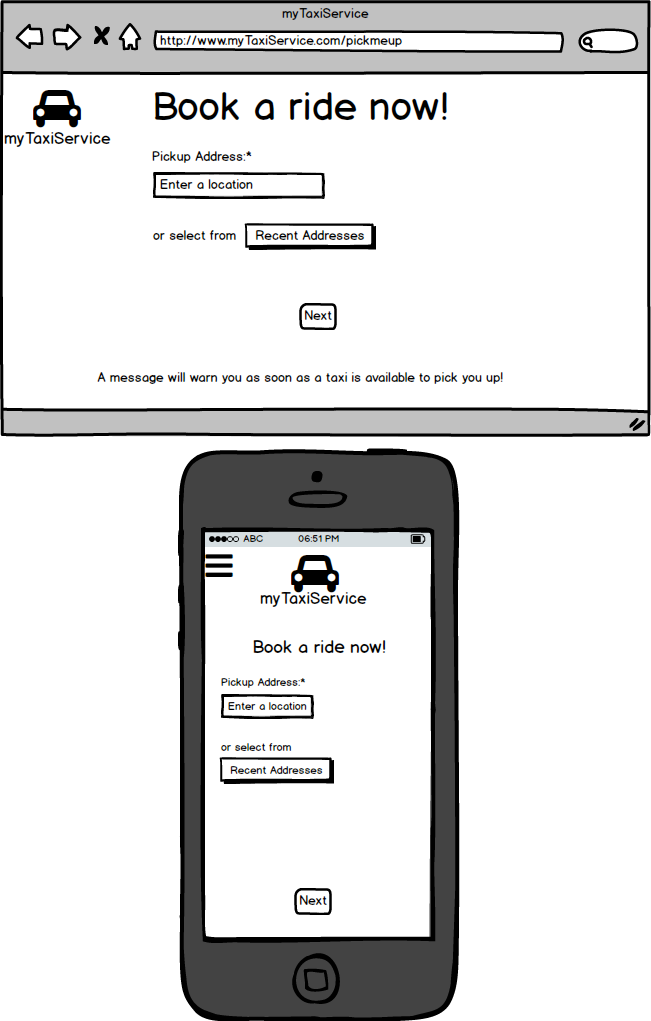
\includegraphics[width=0.9\linewidth]{Pictures/BookARide}
	\end{center}
	
	\pagebreak
	
	\paragraph{Plan a ride} The user can plan a ride in advance providing the pickup and drop off locations, the date and time, the willingness to share the ride.
	
	\paragraph{Your reservations} The user can see both the active reservations and the past ones. The user can edit the active reservations within the established time frame before the meeting time.
	
	\paragraph{Your profile} The user can edit the personal profile modifying the password, phone number, email address, payment method.
	
	\paragraph{Your work} The taxi driver's home page: s/he can accept or reject the requests forwarded by the system. There is also the possibility to inform the system about an ``emergency situation'' and the impossibility to carry out the scheduled jobs. \textcolor{red}{does the system also offer a sat nav function to the driver? in this case do we need two pages, one to accept the job and one related to the current work and map?}
	
	\subsubsection{Hardware Interfaces} \mts does not require and does not support any additional HW interface, it is enough a compatible smartphones or any supported browser on a computer.
	
	\subsubsection{Software Interfaces} \textcolor{red}{do we have to pretend to use sql, java ee....???}
	
	\subsubsection{Communication Interfaces} \mts uses the TCP transport protocol and HTTP/HTTP over SSL application layer protocol to guarantee the top of the line security on the matter of transmission of private data.
	
	\subsection{Functional Requirements}
	
	\subsubsection{User Class 1}
	
	\subsubsection{User Class 2}
	
	\subsection{Performance Requirements}
	
	\subsection{Design Constraints}
	
	\subsubsection{Standards compliance}
	
	\subsubsection{Hardware limitations}
	
	\subsection{Software System Attributes}
	
	\subsubsection{Reliability}
	
	\subsubsection{Availability}
	
	\subsubsection{Security}
	
	\subsubsection{Maintainability}

	\subsubsection{Portability}
	
	\subsection{Other Requirements}
	
	
\end{document}